\section{Prototyp algorytmu}
Po zapoznaniu z wiadomościami teoretycznymi i ustaleniu zakresu projektu, przystąpiono do zaprojektowania prototypów algorytmów $kNN$ oraz $eNN$ w środowisku Matlab.

Algorytm badany był przy użyciu zbioru sygnałów $EKG$ zredukowanych do opisu cech zespołów $QRS$, uporządkowanych do zbioru trzynastu klas. Pierwsza klasa oznaczała normalny zespół QRS, natomiast pozostałe opisują szereg nieprawidłowości pracy serca.
Rozkład danych wejściowych na klasy przedstawiono na rysunku \ref{fig:klasy-danych}.

\begin{figure}[H]
	\centering
	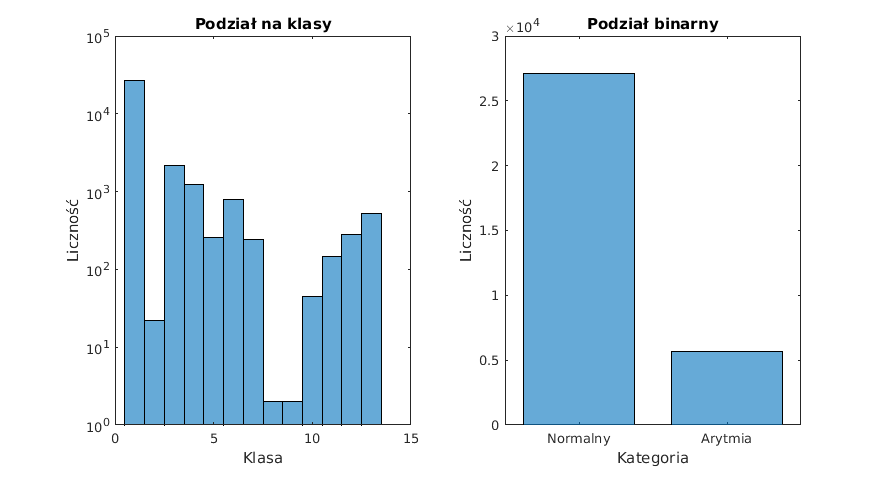
\includegraphics[width=18cm]{img/licznosc_klas}
	\caption{Rozkład danych wejściowych na klasy.}
	\label{fig:klasy-danych}
\end{figure}
Dane zawarte w zbiorze pomiarów nie składają się na klasy o równej liczności. Najliczniejsza klasa zawiera wektory opisujące normalne zespoły QRS. Kategoria ta składa się na $82.67\%$ wszystkich danych. Część klas opisujących nieprawidłowości reprezentowana jest przez zaledwie kilka lubi kilkadziesiąt wektorów cech, co uniemożliwia zaprojektowanie poprawnych klasyfikatorów.

Dane wejściowe poddano normalizacji, która opisana jest równaniem \ref{eq:normalize-data}.

\begin{equation}
\label{eq:normalize-data}
x_j = \frac{x_j - \mu(x_j)}{\sigma(x_j)}, j=1,2...N
\end{equation}
gdzie $x_j$ opisuje $j$-tą kolumnę macierzy danych.

Skuteczność badano niezależnie dla każdego pliku. Wyniki przedstawiono w tabeli \ref{tab:matlab-skutecznosc}. Przyjęto $K=3$. Zmierzono również czas wykonania algorytmów dla wszystkich plików.

\begin{table}[H]
	\centering
	\begin{tabular}{|c|r|r|r|r|}
		\hline

		$Plik$ & Skuteczność & Czas wykonania [s] & Skuteczność & Czas wykonania [s] \\
		\hline
100 & 100.00\% & 0.0567 & 99.69\% & 0.1448 \\ 
\hline
101 & 100.00\% & 0.0182 & 99.51\% & 0.0763 \\ 
\hline
102 & 93.96\% & 0.0159 & 88.46\% & 0.0544 \\ 
\hline
103 & 100.00\% & 0.0151 & 100.00\% & 0.0531 \\ 
\hline
104 & 95.83\% & 0.0063 & 89.58\% & 0.0267 \\ 
\hline
105 & 99.80\% & 0.1218 & 99.59\% & 0.2998 \\ 
\hline
106 & 99.36\% & 0.0362 & 99.36\% & 0.1050 \\ 
\hline
108 & 96.88\% & 0.0015 & 96.88\% & 0.0065 \\ 
\hline
109 & 99.42\% & 0.0129 & 98.25\% & 0.0418 \\ 
\hline
111 & 100.00\% & 0.0069 & 100.00\% & 0.0153 \\ 
\hline
112 & 100.00\% & 0.0920 & 100.00\% & 0.2858 \\ 
\hline
113 & 99.56\% & 0.0223 & 98.69\% & 0.0635 \\ 
\hline
118 & 83.87\% & 0.0024 & 51.61\% & 0.0044 \\ 
\hline
119 & 99.18\% & 0.0247 & 99.18\% & 0.0711 \\ 
\hline
121 & 100.00\% & 0.0148 & 100.00\% & 0.0381 \\ 
\hline
122 & 100.00\% & 0.0546 & 100.00\% & 0.1585 \\ 
\hline
124 & 95.26\% & 0.0201 & 54.98\% & 0.0584 \\ 
\hline
200 & 97.22\% & 0.0039 & 94.44\% & 0.0099 \\ 
\hline
201 & 51.72\% & 0.0017 & 51.72\% & 0.0033 \\ 
\hline
202 & 99.37\% & 0.0112 & 93.08\% & 0.0298 \\ 
\hline
203 & 100.00\% & 0.0389 & 100.00\% & 0.1147 \\ 
\hline
205 & 99.76\% & 0.0585 & 99.76\% & 0.1814 \\ 
\hline
208 & 96.25\% & 0.0304 & 92.13\% & 0.0843 \\ 
\hline
209 & 94.07\% & 0.0072 & 95.76\% & 0.0175 \\ 
\hline
210 & 99.64\% & 0.0926 & 99.46\% & 0.2921 \\ 
\hline
212 & 100.00\% & 0.0148 & 100.00\% & 0.0420 \\ 
\hline
213 & 95.14\% & 0.1684 & 91.36\% & 0.5647 \\ 
\hline
214 & 96.36\% & 0.0069 & 95.45\% & 0.0171 \\ 
\hline
215 & 100.00\% & 0.0139 & 100.00\% & 0.0374 \\ 
\hline
217 & 92.42\% & 0.0035 & 93.94\% & 0.0085 \\ 
\hline
219 & 99.76\% & 0.0556 & 97.56\% & 0.1720 \\ 
\hline
221 & 99.24\% & 0.0084 & 99.24\% & 0.0212 \\ 
\hline
222 & 87.35\% & 0.0567 & 80.54\% & 0.1773 \\ 
\hline
223 & 90.62\% & 0.0015 & 90.62\% & 0.0033 \\ 
\hline
228 & 99.34\% & 0.0343 & 98.68\% & 0.1012 \\ 
\hline
231 & 99.48\% & 0.0490 & 99.21\% & 0.1531 \\ 
\hline
233 & 99.74\% & 0.0499 & 98.95\% & 0.1525 \\ 
\hline
234 & 100.00\% & 0.1131 & 100.00\% & 0.3537 \\ 
\hline

		
	\end{tabular}
	\caption{Wyniki pracy algorytmu kNN i eNN w środowisku Matlab.}
	\label{tab:matlab-skutecznosc}
	
\end{table}

Wyniki otrzymane za pomocą algorytmów $kNN$ oraz $eNN$ są zbliżone do siebie z lekką przewagą na korzy algorytmu $kNN$. Duży wpływ na działanie algorytmów miał podział próbek w zbiorze uczącym na poszczególne klasy. Znaczna przewaga danych należących do klasy 1 miała negatywny wpływ na skuteczność klasyfikacji, co jest uzasadnione w przypadku korzystania z metod statystycznych. W optymalnie przygotowanym zbiorze uczącym próbki powinny być równomiernie rozłożone na wszystkie klasy. Czas wykonania algorytmu $eNN$ jest zwykle około trzykrotnie dłuższy niż w przypadku algorytmu $kNN$. Bardzo ważne okazało się zastosowanie obliczeń wektorowych, które są bardzo dobrze zoptymalizowane w środowisku Matlab i cechują się znacznie większą wydajnością niż podejście iteracyjne. W przypadku algorytmu $eNN$ różnice w czasie obliczeń przekraczały trzy rzędy wielkości.